


\tableofcontents
\chapter*{Introduction}

\tria est un logiciel permettant d'identifier facilement des lieux de problèmes dans des situations relationnelles courantes. Ces situations ont été schématisées au préalable et le but de \tria est de fournir un accès facile et rapide aux informations qui intéressent le plus l'utilisateur.\\

Dans un deuxième temps, \tria permet d'exporter les schémas importants sous la forme d'images afin de les utiliser dans le cadre d'une présentation ou d'un rapport. Il est possible de fortement personnaliser l'apparence des schémas lors de ces exportations pour les adapter au cadre d'utilisation.\\

L'utilisation classique se déroule de la manière suivante :\\
\begin{enumerate}
\item Création d'une session, l'utilisateur choisi dans une liste l'ensemble des acteurs concernés par la situation sur laquelle il veut travailler. Il est possible de saisir les deux récits des différents acteurs lors de cette étape.\\
\item Navigation dans les différentes situations impliquant ces acteurs. Un système de navigation permet a l'utilisateur d'accéder à l'ensemble des briques pouvant l'intéresser (chaque brique correspond à une situation réelle). Un classement permet à l'utilisateur de se concentrer en premier sur les briques qui sont à priori les plus intéressantes.\\
\item L'utilisateur saisi les relations liants les différents acteurs dans chaque situation. Le logiciel met alors en avant les relations en écart avec une situation théorique correcte.\\
\item Une fois ces lieux identifiés, l'utilisateur exporte les schémas concernés vers des images en mettant en valeur les lieux de problèmes. Ces images permettront de faciliter la résolution des problème en accélérant la compréhension des mécanismes sous-jacent.\\
\end{enumerate}



\begin{figure}[h!t]
\centering
\Ovalbox{
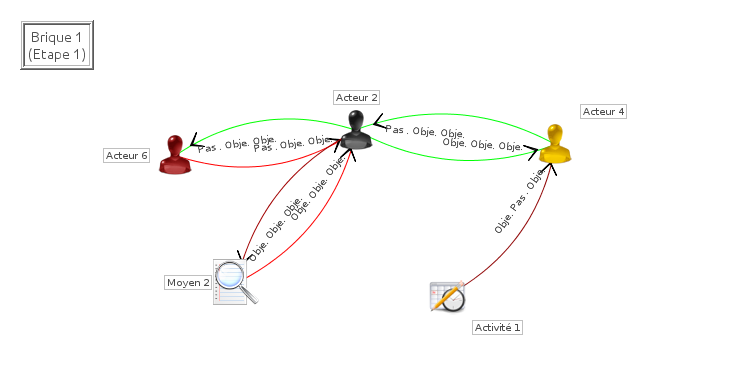
\includegraphics[width=12cm]{images/exportOrigin.png}
}
\caption{Une brique lors de l'édition de ses relations}
\vspace*{15pt}
\Ovalbox{
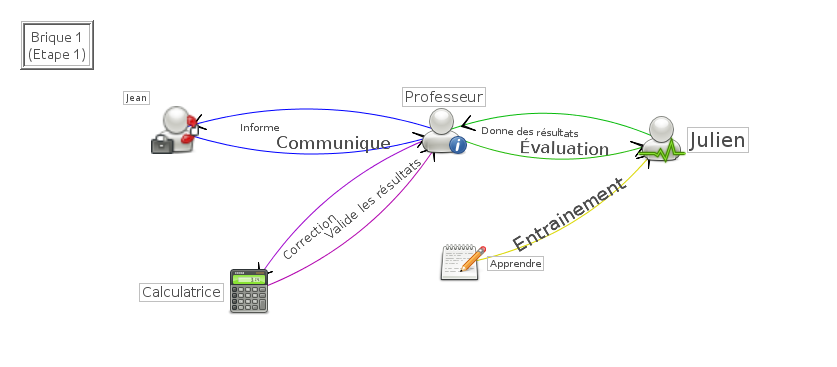
\includegraphics[width=12cm]{images/exportModifie.png}
}
\caption{La même une fois personnalisée afin d'être exportée.}


\end{figure}
